%%=============================================================================
%% Inleiding
%%=============================================================================
\chapter{Inleiding}
\label{ch:inleiding}
Het onderzoek zal verschillende methodes voor offline opslag en synchronisatie analyseren en onderzoeken. Het onderzoek zal van elke methode de voor- en nadelen overlopen. In de sectie ~\ref{sec:business-case} 'Business case' wordt de business case van Pridiktiv.care - into.care toegelicht. Daarna worden in sectie ~\ref{sec:terminologie} 'Terminologie' de verschillende relevante termen overlopen. In sectie ~\ref{sec:stand-van-zaken} 'Stand van zaken' komt de context en noodzaak van het onderzoek aan bod. Tenslotte volgt de probleemstelling, de onderzoeksvraag en de opzet van de bachelorproef.
%% literatuurstudie. Vergeet niet telkens je bronnen te vermelden!
\section{Business Case}
\label{sec:business-case}
\subsection{Voorstelling bedrijf}
Pridiktiv - into.care is een start-up die een mobiel platform aanbiedt aan zorgverstrekkers om de administratielast te verlichten. Op die manier is er meer tijd voor zorg en verliezen de zorgverleners minder tijd bij het invullen van documenten. UX\footnote{UX staat voor User Experience. Een verzamelnaam die alle emoties capteert die gebruikers ervaren bij het gebruiken van een product.} en mobile vormen de speerpunten van de business doelstellingen en vormen de belangrijkste factoren om zich te onderscheiden van andere concurrenten. Op termijn wil de start-up een modern, mobile-friendly ERP-systeem aanbieden aan woonzorgcentra.
\subsection{Context en probleemstelling van de business case}
De applicatie draait op een smartphone in een woonzorgcentrum. Het woonzorgcentrum beschikt over draadloos internet maar de internetdekking in het gebouw is niet volledig. Dus moet de applicatie ook offline werken. Wanneer verschillende waarden worden geregistreerd met de applicatie (zoals bloeddruk, gewicht, inname medicatie) worden die offline opgeslagen in een IndexedDB. Wanneer het toestel terug online komt, moeten deze waarden worden doorgestuurd naar de backend. Het is essentieel dat er geen data verloren gaat aangezien het gaat om medische data. Bij de start van het onderzoek gebruikte de applicatie een algoritme die een HTTP call uitvoert wanneer een waarde wordt ingegeven. Wanneer dit niet lukt, veronderstelt het algoritme dat de applicatie offline is en worden de data lokaal opgeslagen. Wanneer het toestel terug online komt, dan worden de offline data gesynchroniseerd met de server. De realiteit wijst echter uit dat betrouwbaar internet eerder uitzonderlijk is in een woonzorgcentrum. In deze context is er dus nood aan een 'offline first' -  oplossing.
\subsection{De Pridiktiv applicaties en technologiestack}
Pridiktiv maakt gebruik van verschillende applicaties om de business doelstellingen te realiseren. In hoofdstuk ~\ref{ch:setup} kan u een gedetailleerd bespreking terugvinden van de verschillende applicaties.
\subsubsection{Client: Mobile applicatie}
De huidige applicatie is een Angular\footnote{Wanneer de term 'Angular' wordt gebruik zonder versienummer, dan duidt dat op alle versies vanaf Angular 2. AngularJS is de verwijzing naar de 'oude' Angular versie} applicatie met Redux als state container. Voor lokale opslag wordt momenteel gebruik gemaakt van Mozilla's localForage\footnote{localForage maakt gebruik van de verschillende DOM Storage methodes en voorziet een uniforme interface voor het opslaan van data in de browser.} library. De applicatie is gebundeld als een Cordova applicatie.
\subsubsection{Client: Backoffice applicatie}
De backoffice applicatie is net als de mobiele applicatie een Angular applicatie maar dan gericht voor desktop gebruik. Synchronisatie en caching is voor deze applicatie niet relevant. Deze applicatie komt niet verder aan bod in dit onderzoek
\clearpage
\subsubsection{Server side: Serverless architectuur}
De backend van de businesscase maakt gebruik van een serverless architectuur in de Amazon Web Services Cloud en bestaat uit een verzameling van verschillende microservices die AWS\footnote{AWS is de afkorting voor Amazon Web Services. Gemakkelijkheidshalve wordt in dit onderzoek AWS gebruikt om te verwijzen naar AWS} Lambda gebruiken. Om de data te persisteren wordt DynamoDB van AWS gebruikt.
\section{Terminologie}
\label{sec:terminologie}
In deze sectie komen de verschillende begrippen met betrekking tot de componenten van het onderzoek, het prototype en tools aan bod. De volledige lijst met begrippen en termen kan u terugvinden onder het hoofdstuk 'Glossarium'. Er is een minimum kennis in verband met software ontwikkeling vereist van de lezer om deze sectie volledig te begrijpen.
\subsection{Huidige Web APIs voor lokale opslag}
Er zijn momenteel 4 APIs \autocite{mozilla-overview} voor lokale opslag die ondersteund worden door verschillende browsers. Deze APIs worden ondersteund \autocite{WHATWG-storage-API} door de Web Hypertext Application Technology Working Group, aangegeven door WHATWG. De specificatie van de API wordt dan gestandardiseerd door het World Wide Web Consortium, aangegeven door W3C. Dit proces is belangrijk omdat de APIs dan door de populaire browsers zoals Chrome, Firefox en Safari worden ge\"integreerd. Op die manier kunnen webapplicaties gebruik maken van de verschillende APIs. Het is belangrijk om deze APIs kort te overlopen omdat ze steeds gebruikt worden bij de verschillende caching technieken om data lokaal op te slaan.
\subsection{Web Storage}
localStorage en sessionStorageAPIs vallen onder Web Storage of DOM Storage \autocite{clientside-storage}. Wanneer de browser ondersteuning biedt voor Web Storage, zijn beide beschikbaar op het globale window. Web Storage wordt vaak vergeleken met cookies. Terwijl die vergelijkbaar zijn in functie, verschilt Web Storage in volgende aspecten: 
\begin{itemize}  
\item Opslag ruimte: Afhankelijk van browser maar meestal 5 MB beschikbare opslagruimte in vergelijking met maar 4 kb voor cookies.
\item Client-side interface: Cookies kunnen zowel door server als client side worden gebruikt. Web storage valt exclusief onder client-side scripting.
\item Twee verschillende storage omgevingen: localStorage en sessionStorage.
\item Een eenvoudigere programmeerbare interface in vergelijking met cookies.
\end{itemize}
\clearpage
\subsubsection{localStorage}
Data die in localStorage wordt opgeslagen is persistent tenzij die manueel wordt verwijderd door de gebruiker of applicatie. localStorage is dus een belangrijke kandidaat om data lokaal op te slaan in geval een applicatie offline moet kunnen worden gebruikt. Bij gevoelige data zoals medische data is het belangrijk om de data te verwijderen uit de localStorage wanneer die niet meer moet worden gecached.
\subsubsection{sessionStorage}
Het grote verschil \autocite{mozilla-overview} met localStorage is dat sessionStorage een vervalttijd heeft en de inhoud van de sessionStorage wordt verwijderd wanneer de sessie vervalt. Een sessie vervalt bijvoorbeeld hij het openen van een nieuw tabblad of browser venster. Refreshen van de browser heeft geen impact op de sessionStorage. sessionStorage laat toe om instances van een webapplicatie te runnen in verschillende browser windows, zonder dat er conflicten optreden.
\subsubsection{lndexedDB}
IndexedDB \autocite{indexeddb-moz} is een Web API die gebruikt wordt het opslaan van relatief grote data structuren in browsers. Dankzij indexering is het mogelijk om sneller en performanter \autocite{clientside-storage} te zoeken in de databank in vergelijking met localStorage en sessionStorage. Net zoals SQL-databanken is IndexedDB een transactional database system. Het grote verschil is echter het gebruik van JSON objecten in plaats van fixed columns tables om data op te slaan, vergelijkbaar met andere NoSQL databanken zoals MongoDB of CouchDB. Onder impuls van Mozilla wordt IndexedDB waarschijnlijk de alternatieve storage standaard voor het web in de nabije toekomst.
\subsubsection{Web SQL - deprecated}
Net zoals bij IndexedDB biedt Web SQL toegang tot een databank waar data structuren kunnen worden opgeslagen. Met een SQL variant is het dan mogelijk om queries uit te voeren op de Web SQL database. Momenteel biedt enkel SQLite een database systeem voor Web SQL. W3C werkt momenteel niet meer verder aan de specificatie \autocite{websql-specification} van Web SQL omdat er te weinig onafhankelijke implementaties zijn van Web SQL. Het gebruik van Web SQL wordt sterk afgeraden door het deprecated status\footnote{'Deprecated' binnen de context van softwareontwikkeling wil aangeven dat de functionaliteit niet meer verder wordt ondersteund of ontwikkeld} en wordt niet gebruikt in het onderzoek en de business case.
\clearpage
\subsection{Scalable Angular Architecture}
\begin{figure}[h]
\caption{Overzicht van een schaalbare web applicatie}
\centering
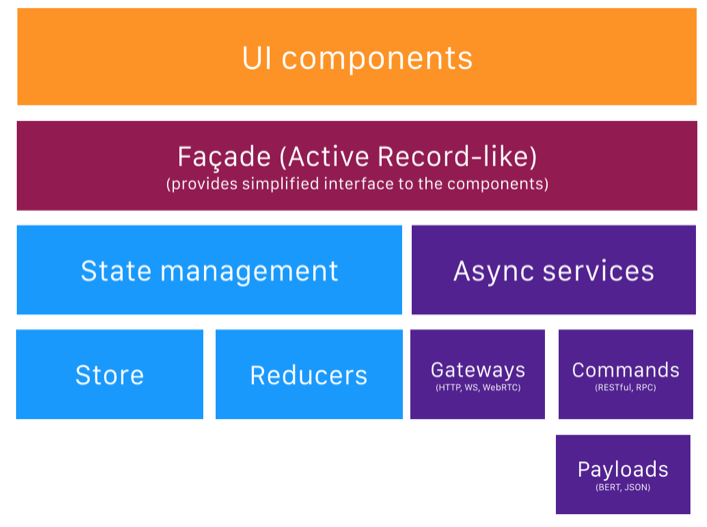
\includegraphics[width=0.8\textwidth]{scalable-webapplication}
\end{figure}
Bij de start van de ontwikkeling van een Angular applicatie is het belangrijk om na te denken over de architectuur \autocite{minko-gechev-scalable} van de applicatie. Moderne SPA-technologie\"en zoals React en Angular maken gebruik van components. Een component is combinatie van HTML, JavaScript en optioneel CSS. Door alles in componenten onder te verdelen is het eenvoudiger om de applicatie te onderhouden omdat alle relevante data word gegroepeerd. Componenten zelf kunnen 'dumb' zijn als ze enkel data voorstellen of 'smart' wanneer ze data opvragen of verwerken.

De dataflow tussen componenten is ook belangrijk om een beheersbare \autocite{brechtbilliet-scalable} applicatie te bouwen. Zo communiceren child components enkel maar met hun parent en interageert een parent met een model dat op zijn beurt communiceert met een 'store'\footnote{Zie ~\ref{subsec:reactive-programming} Redux store: een state container} aan de hand van acties. Wanneer de state wordt gewijzigd in de store, dan wordt de volledige component tree opnieuw ge\"evalueerd. Een ander belangrijk aspect van een scalable SPA is het inperken van de communicatiemogelijkheden van smart components. Door het gebruik van een extra abstractie layer, zoals een model of sandbox, is het mogelijk om de communicatie te verwerken in de abstractielaag en op die manier een microservice te genereren die gemakkelijk kan worden refactored indien er aanpassingen moeten gebeuren.
\clearpage
\subsection{Redux store: een state container}
Redux store is een container die de state van de applicatie bijhoudt waarbij performantie en consistentie centraal staan. De redux store is de 'single source of truth', verder benoemd als SSOT, voor de applicatie en moet ervoor zorgen dat de data van alle componenten consistent is met elkaar en er geen duplicate data is. Alle updates aan de data worden eerste weggeschreven naar de store en daarna gecachet. In het geval dat de gebruiker toegang heeft tot het Internet worden de data verstuurd naar de achterliggende systemen. Indien er geen of slechte internetverbinding is, krijgt de user de gecachte data te zien dankzij de SSOT. De store werkt met volgende \autocite{ngrx-info} principes :
\begin{itemize}  
\item de state is een single immutable JSON data structure, alle aanpassingen in de state cree\"eren een nieuwe state die de oude state overschrijft
\item trigger of dispatch events initialiseren acties in de reducers
\item reducers verwerken acties en wijzigen de state door een nieuwe state te cree\"en. Een reducer is een idempotente\footnote{Een idempotente functie is een functie die een operatie uitvoert zonder neveneffecten als die meerdere keren met dezelfde input wordt opgeroepen} functie die een actie moet verwerken
\item de state van de store kan asynchroon worden opgevraagd
\end{itemize}
In de applicatie van de business case wordt er gebruikt gemaakt van een Angular implementatie van Redux, de ngrx store. Net als Angular maakt ngrx gebruikt van RxJS. Zo is het mogelijk om RxJS componenten zoals Observables en Subjects te gebruiken bij het opvragen van de state.
\begin{figure}[h]
\caption{Voorbeeld van de flow bij een dispatch in Redux}
\centering
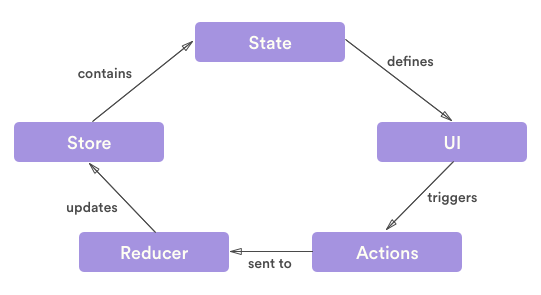
\includegraphics[width=0.9\textwidth]{ui_workflow}
\end{figure}
\clearpage
\subsection{Reactive programming paradigm}
\label{subsec:reactive-programming}
Het reactive programming paradigm \autocite{reactivex-intro} is gebouwd rond veranderende data flows, waarbij een applicatie kan reageren op nieuwe of andere input. Dankzij de ReactiveX library is het mogelijk om in verschillende programmeertalen componenten van reactive programming te gebruiken. De library laat toe om asynchroon en event-driven applicaties te ontwikkelen, die in real-time data kunnen manipuleren en tonen. Het breidt het Observer design pattern uit waarbij het mogelijk is om verschillende operators te 'chainen' met elkaar zonder rekening te houden met low level concerns zoals threading, synchronisatie, thread safety, concurrent data structures en blocking I/O. De RxJS library van ReactiveX is volledig ge\"integreerd in Angular en ngrx store.

Met Promises \autocite{promise-info} was het reeds mogelijk om asynchroon te programmeren in JavaScript dus wat zijn de voordelen van RxJS ten opzicht van promises in JavaScript? Een Promise kan maar een enkel event afhandelen en kan niet worden gestopt. Een Observable kan worden beschouwd als een stream van events waarop verschillende manipulaties zoals map, reduce en filter kunnen worden op toegepast.
\begin{lstlisting}[caption=Voorbeeld de mapTo operator in RxJS]
// een event wordt elke 2 seconden gegenereerd
const source = Rx.Observable.interval(2000);
// mappen van elke event naar 'Hello World' string
const example = source.mapTo('HELLO WORLD!');
// subscriben op operator om waarden te ontvangen
const subscribe = example.subscribe(val => console.log(val));
//output: 'HELLO WORLD!'...'HELLO WORLD!'...'HELLO WORLD!'...

\end{lstlisting}
\subsection{Offline First}
'Offline First' is een stroming \autocite{offline-first} binnen web development waarbij offline gebruik als de basis wordt beschouwd van de applicatie. Net zoals bij 'Progressive Enhancement' wordt online functionaliteit beschouwt als een extra laag van features die de applicatie kan aanbieden. Het idee is gegroeid vanuit de teleurstelling dat 'always online' omwille van technische, geografische, financi\"ele en praktische redenen nog niet haalbaar is voor de nabije toekomst.
\clearpage
\subsection{Amazon Web Services}
De applicaties en backend van de business case maken uitgebreid gebruik van Amazon Web Services (AWS). Volgende componenten komen aan bod in het onderzoek:
\begin{itemize}
\item Amazon SQS: Simpelweg Simple Queue Service is een message queue service die verschillende AWS services toelaat om data te plaatsen in een queue. SQS voorziet 2 varianten. De standard queue biedt de snelste en meer performante oplossing maar hanteert geen FIFO-principe. Een FIFO-queue, zoals de naam reeds aangeeft, hanteert wel het FIFO-principe en elke message in de queue wordt altijd maar 1 keer geleverd. Andere AWS services kunnen de queue pollen voor nieuwe data.
\item Lambda: Met AWS Lambda is het mogelijk om code, functies en operaties uit te voeren in de cloud dus zonder servers zelf te beheren en vormt de basis voor de serverless architectuur. De input voor de functie kan worden geleverd door HTTP endpoints maar ook door andere AWS services en is een voorbeeld van een event-driven architectuur. De output kan dan bijvoorbeeld worden gepersisteerd in DynamoDB of teruggestuurd worden naar de client. De verschillende Lambda functies vormen de microservice architectuur in de backend van de businesscase.
\item Amazon SNS: Amazon Simple Notification Service is een push notificatie service die toelaat om berichten te sturen naar mobiele toestellen, email adressen of andere AWS services. Met SNS is het onder andere mogelijk om polling van andere services te vermijden.
\item DynamoDB: DynamoDB is een fully-managed\footnote{fully-managed houdt in dat dat het management en beheer van een service of databank wordt 'outsourced' naar de service provider. In het geval van DynamoDB moet de developer zich niet meer bezighouden met installatie, upgrades, provisioning, deployment, backups, restores en database availability.} NoSQL database van AWS en wordt gebruikt door de business case voor de data opslag. DynamoDB voorziet geen automatische synchronisatie met clients.
\item API Gateway: API Gateway is een fully managed service die toelaat om de toegang tot API's te beheren.
\end{itemize}
\section{Stand van zaken}
\label{sec:stand-van-zaken}
Wanneer een ontwikkelaar de eindgebruiker van zijn web -of mobiele applicatie wil voorstellen, dan denkt hij vaak aan een gebruiker met dezelfde eigenschappen als zichzelf (laatste smartphone, up-to-date besturingssysteem,  snelle internet verbinding). De ontwikkelomgeving (snelle desktop/laptop met een betrouwbare en snelle internet verbinding) simuleert amper de omgeving van de eindgebruiker \autocite{chrome-offline-first-statement}. Bepaalde omgevingsfactoren zoals tunnels, trein en vliegtuig hebben een grote invloed op de betrouwbaarheid van de connectie. Het klassieke client - server model waarbij de client enkel maar als het ware een view is van de data die door de server worden bijgehouden, is achterhaald, want elke onderbreking in de internetconnectie zorgt ervoor dat de applicatie niet meer kan worden gebruikt.
\clearpage
Meeste mobiele- en webapplicaties hebben twee momenten waarbij er problemen kunnen optreden door de status van de connectie:
\begin{enumerate}  
\item client stuurt request naar de server
\item server pusht request naar client
\end{enumerate}
Afhankelijk van de business context van de applicatie, zijn er verschillende mogelijkheden:
\begin{itemize}  
\item De gebruiker al dan niet op de hoogte brengen van veranderingen in de status van de connectie. Bijvoorbeeld: bij het versturen van een bericht kan de gebruiker op de hoogte worden gebracht dat het bericht pas wordt verstuurd wanneer de applicatie terug online is.
\item Offline client-side creatie en manipulatie van data toelaten aan de hand van caching. Wanneer de applicatie terug online, deze data synchroniseren met de server.
\item Uitschakelen of aanpassen van bepaalde features wanneer de applicatie offline is.
\end{itemize}
Daarnaast is het mogelijk dat de server data wil pushen naar de applicatie van de gebruiker omdat deze door een andere client werd gewijzigd. De applicatie moet de gebruiker dan waarschuwen dat er nieuwere, recentere data beschikbaar zijn en indien nodig, een conflict-resolution aanbieden. Momenteel zijn er al enkele frameworks en databank systemen die toelaten om (offline) automatisch data te synchroniseren van een web- of mobiele applicatie met de achterliggende databank. CloudBoost, CouchBase en Firebase bieden een all-in-one oplossing. Deze oplossing is echter niet compatibel met de bestaande backend. Daarom komen deze opties dan ook niet meer verder aan bod in het onderzoek.
%% TODO: deze sectie (die je kan opsplitsen in verschillende secties) bevat je
\section{Probleemstelling en Onderzoeksvragen}
\label{sec:onderzoeksvragen}
Het doel van dit onderzoek is het ontwerpen van een algoritme of architectuur die compatibel is met de huidige applicaties en technologie stack. Hoe wordt conflict-resolution opgelost en moet de gebruiker daar zelf een keuze maken of kan de applicatie of achterliggende systemen zelf alle conflicten oplossen? Het is de intentie van het onderzoek om tot een betrouwbare oplossing te komen voor het probleem van de business case. Zoals reeds vermeld moet in het geval van de business case, de applicatie zonder onderbreking gemakkelijk kunnen overstappen van een offline status naar een online status en omgekeerd, zonder dat er daarbij belangrijke data verloren gaat. De applicatie werkt met vertrouwelijke medische data waardoor het verlies van data onaanvaardbaar.

%% TODO:
%% Uit je probleemstelling moet duidelijk zijn dat je onderzoek een meerwaarde
%% heeft voor een concrete doelgroep (bv. een bedrijf).
%%
%% Wees zo concreet mogelijk bij het formuleren van je
%% onderzoeksvra(a)g(en). Een onderzoeksvraag is trouwens iets waar nog
%% niemand op dit moment een antwoord heeft (voor zover je kan nagaan).
\clearpage
\section{Opzet van deze bachelorproef}
\label{sec:opzet-bachelorproef}

%% TODO: Het is gebruikelijk aan het einde van de inleiding een overzicht te
%% geven van de opbouw van de rest van de tekst. Deze sectie bevat al een aanzet
%% die je kan aanvullen/aanpassen in functie van je eigen tekst.

De rest van deze bachelorproef is als volgt opgebouwd:

In het volgende hoofdstuk~\ref{ch:methodologie} wordt de methodologie toegelicht die werd gehanteerd voor dit onderzoek. De applicatie van de business case, backend infrastructuur voor dit onderzoek worden toegelicht in hoofdstuk~\ref{ch:setup}. Het onderzoek start in hoofdstuk~\ref{ch:synchronisatiemethdodes} met een opsomming van verschillende synchronisatie mogelijkheden. In hoofdstuk~\ref{ch:onderzoek} worden de oplossingen op de verschillende problemen bij synchronisatie overlopen. Tenslotte kan u in hoofdstuk~\ref{ch:conclusie} de conclusie en een oplossing vinden. Daarbij wordt ook een aanzet gegeven voor toekomstig onderzoek binnen dit domein. Indien bepaalde begrippen onduidelijk zijn, vindt u een beknopte uitleg in het hoofdstuk~\ref{ch:glossarium}.
%% TODO: Vul hier aan voor je eigen hoofstukken, één of twee zinnen per hoofdstuk


